\documentclass[pdftex,11pt,a4paper]{article}\usepackage{graphicx, color}
%% maxwidth is the original width if it is less than linewidth
%% otherwise use linewidth (to make sure the graphics do not exceed the margin)
\makeatletter
\def\maxwidth{ %
  \ifdim\Gin@nat@width>\linewidth
    \linewidth
  \else
    \Gin@nat@width
  \fi
}
\makeatother

\IfFileExists{upquote.sty}{\usepackage{upquote}}{}
\definecolor{fgcolor}{rgb}{0.2, 0.2, 0.2}
\newcommand{\hlnumber}[1]{\textcolor[rgb]{0,0,0}{#1}}%
\newcommand{\hlfunctioncall}[1]{\textcolor[rgb]{0.501960784313725,0,0.329411764705882}{\textbf{#1}}}%
\newcommand{\hlstring}[1]{\textcolor[rgb]{0.6,0.6,1}{#1}}%
\newcommand{\hlkeyword}[1]{\textcolor[rgb]{0,0,0}{\textbf{#1}}}%
\newcommand{\hlargument}[1]{\textcolor[rgb]{0.690196078431373,0.250980392156863,0.0196078431372549}{#1}}%
\newcommand{\hlcomment}[1]{\textcolor[rgb]{0.180392156862745,0.6,0.341176470588235}{#1}}%
\newcommand{\hlroxygencomment}[1]{\textcolor[rgb]{0.43921568627451,0.47843137254902,0.701960784313725}{#1}}%
\newcommand{\hlformalargs}[1]{\textcolor[rgb]{0.690196078431373,0.250980392156863,0.0196078431372549}{#1}}%
\newcommand{\hleqformalargs}[1]{\textcolor[rgb]{0.690196078431373,0.250980392156863,0.0196078431372549}{#1}}%
\newcommand{\hlassignement}[1]{\textcolor[rgb]{0,0,0}{\textbf{#1}}}%
\newcommand{\hlpackage}[1]{\textcolor[rgb]{0.588235294117647,0.709803921568627,0.145098039215686}{#1}}%
\newcommand{\hlslot}[1]{\textit{#1}}%
\newcommand{\hlsymbol}[1]{\textcolor[rgb]{0,0,0}{#1}}%
\newcommand{\hlprompt}[1]{\textcolor[rgb]{0.2,0.2,0.2}{#1}}%

\usepackage{framed}
\makeatletter
\newenvironment{kframe}{%
 \def\at@end@of@kframe{}%
 \ifinner\ifhmode%
  \def\at@end@of@kframe{\end{minipage}}%
  \begin{minipage}{\columnwidth}%
 \fi\fi%
 \def\FrameCommand##1{\hskip\@totalleftmargin \hskip-\fboxsep
 \colorbox{shadecolor}{##1}\hskip-\fboxsep
     % There is no \\@totalrightmargin, so:
     \hskip-\linewidth \hskip-\@totalleftmargin \hskip\columnwidth}%
 \MakeFramed {\advance\hsize-\width
   \@totalleftmargin\z@ \linewidth\hsize
   \@setminipage}}%
 {\par\unskip\endMakeFramed%
 \at@end@of@kframe}
\makeatother

\definecolor{shadecolor}{rgb}{.97, .97, .97}
\definecolor{messagecolor}{rgb}{0, 0, 0}
\definecolor{warningcolor}{rgb}{1, 0, 1}
\definecolor{errorcolor}{rgb}{1, 0, 0}
\newenvironment{knitrout}{}{} % an empty environment to be redefined in TeX

\usepackage{alltt}
\usepackage{natbib}
\usepackage{wrapfig}
\usepackage[font=small,labelfont=bf]{caption}
\usepackage[none]{hyphenat}
\usepackage{tabularx}

\bibliographystyle{ecol_let}
\setlength{\parindent}{0cm}

\addtolength{\textwidth}{3cm}
\addtolength{\hoffset}{-1.5cm}

\addtolength{\textheight}{2cm}
\addtolength{\voffset}{-1cm}




\begin{document}

\title{Understanding range shift model error: The influence of generation time and rate of adaptation on species distribution model predictions.}
 \date{}
\maketitle

{\bf  Working group proposal \\}
Short title: Range shifts and rates of adaptation \\
{\it Submitted to NCEAS on August 31, 2012\\}

{\bf Principle Investigator\\}
Edmund M. Hart\\
Beaty Biodiversity Center\\
Dept. of zoology\\
University of British Columbia\\
4200-6270 University Blvd\\
Vancouver, B.C. V6T 1Z4\\
{\it ehart@zoology.ubc.ca}\\ 



{\bf Project Summary:} Species range shifts is one of the most well documented responses of species to climate change and have been modeled using correlative niche models (species distribution models, SDMs) for more than a decade.  These models are stastical correlations between a species realized niche and abiotic variables, because they ignore ecological theory there is often a difference between predictions and a species' actual distribution (error). One potential source of error is that these models ignore differing rates of adaptation to novel climates.  Our group will seek to understand the source of this error using meta-analysis, and integrate adaptation into range shift theory. However much of the data from these models is locked in the form of published figures and maps. Therefore a second outcome of our working group will be a web-based data extraction tool. This will allow anyone to upload a figure and extract data from it and store it in DataONE.  Beyond producing manuscripts, we will contribute tools for meta-analysis beyond the life of our working group.
\\
\begin{description}\itemsep1pt
\item[Start date] December 2012
\item[End date] December 2013
\item[Data release] December 2013
\item[Resubmission?] No
\end{description}

\pagebreak[4]

\section*{Problem Statement}
Species' range shifts was one of the earliest documented ecological responses to climate change \citep{Parmesan1996,Parmesan1999,Parmesan2003}.  Understanding rang shifts is a pressing issue because as warming increases, species are exhibiting rapid distributional changes \citep{Chen2011}. Since the late 1990's ecologist's have been using species' distribution models (SDM's) to try and predict how those ranges will shift over the next century \citep{Davis1998,Iverson1998,Guisan2000,Peterson2001}. These models assume that the realized niche of a species is primarily determined by climate variables \citep{Austin2002,Dormann2007}.   Early models ignored physiology,  biotic interactions and rapid local adaptation, relying soley on correlations between current distribution and climate variables \citep{Davis1998,Pearson2003,Guisan2005,Helmuth2005}.  Aside from variance due to lack of ecological theory \citep{Elith2009}, SDM's can show great variance in their predictive abilities \citep{Elith2006,Kearney2009,Elith2010}.  More recent SDM's have begun to incorporate mechanisms such as physiology \citep{Crozier2006,Buckley2010,Buckley2011} and  life history traits \citep{Midgley2006,Kearney2009,Poyry2009,Angert2011a} to improve fit. Including traits and physiology offers a significant improvement in model predictions \citep{Angert2011a,Buckley2011} but still only explain small percentage of variance.  Other factors may be important in explaining the error in species actual ranges and their predicted distribution such as biotic interaction and adaptation. \\ 

\begin{wrapfigure}{r}{.5\textwidth}
\begin{knitrout}
\definecolor{shadecolor}{rgb}{0.969, 0.969, 0.969}\color{fgcolor}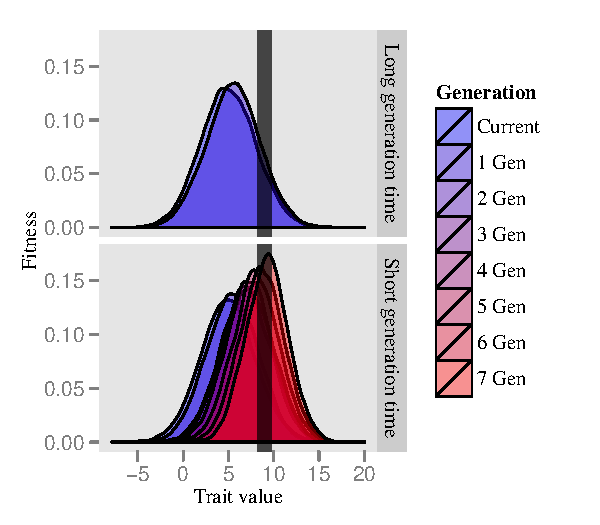
\includegraphics[width=\maxwidth]{figure/add_demo} 
\end{knitrout}

\caption{ \footnotesize{ \textit{A species with a long generation time can only complete 1 generation in a fixed time, but a short generation time can complete 7 in the same time period, rapidly advancing towards the new fitness optimum (black line)  }}\label{fig:add_demo}}
\end{wrapfigure}
Adaptation is important to understanding how species will respond to climate change \citep{Visser2008,lavergne2010biodiversity,Hoffmann2011}, but is difficult to accurately measure in the field \citep{Hansen2012}.
Despite adaptation playing an important role in species range shifts to both current \citep{Thomas2001,Bridle2007} and historical climate change \citep{Davis2001} it is conspicuously absent from SDMs \citep{Hoffman2011} (but see \citet{Kearney2009a}).  
Shorter generation times allow for a more rapid adaptive response to strong selective pressures \citep{Berteaux2004,Somero2010,Hoffmann2011,Reed2011,Shaw2012,Walters2012}.  The first reason is that species with shorter generation times can make use of standing additive genetic variation (Figure 1). Models of population persistence have demonstrated that shorter generation times can allow populations to persist by novel adaptation \citep{Gomulkiewicz1995, Hoffmann2011}. For instance fur seals are predicted to be unable to adapt to rapid climate change because of long generation times, but this is not the case for other antartic species with short generation times \citep{Forcada2008}. One consequence of strong directional selection is the loss of additive genenetic variance necessary for adaptation \citep{Lande1996,Hoffmann2011}.  However, species with shorter generation times also have higher rates of molecular evolution due to increased mutation rates \citep{Thomas2010} adding to the total additive genetic variance.  The expecation is species with short generation times will track their climate on the expanding front of the range, but not necessarily go extinct at the trailing edge, instead adapting to novel climate conditions. Therefore one of the fundamental assumptions of SDMs, that species will track their current climate conditions as they shift latitudinally, can be violated by species with short generation times. \\

\textbf{Our goal is to (1) quantify SDM error across a range of taxa, (2) investigate how rates of adaptation introduce error model prediction, and  (3) build tools to automatically extract data from figures in the published literature.}
\section*{Proposed Activities}

Despite more than a decade of publications on SDM's, adaptation is still absent from most models \citep{Kearney2009}. We want to analyze the large number of existing SDMs and attempt to integrate adaptation into range shift theory. By calculating a standard metric of error it is possible to construct models of that unexplained deviance from actual distributions.  The challenge is that much of the data for these models is locked in the form of published figures.  Methods already exist for data extraction such as the \textit{digitize} package \citep{Poisot2011} for R (Figure 2). 

\begin{figure}[!h]
\centering
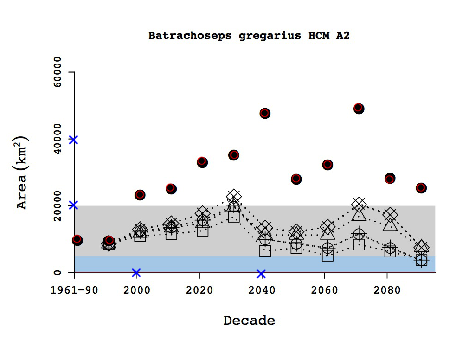
\includegraphics[height=2.2in,width=2.7in]{ExtractPlot.png}
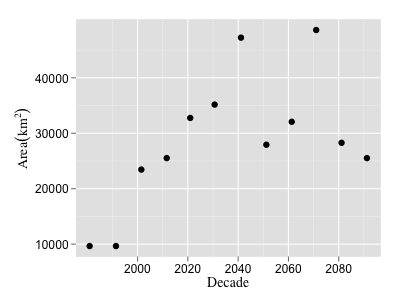
\includegraphics[height=2.2in,width=2.7in]{exportdat.png}
\caption{\textbf{Left panel: }\textit{Range shift predictions fram \citet{Early2011a} of} Batrachoseps gregarius \textit{ with calibration points marked} \textbf{Right panel: } \textit{Extracted data points using the digitize package for R \citep{Poisot2011}}}

\end{figure}
Using a combination of JavaScript and Python, we want to implement a web based interface for the extraction of data from a variety of figure types in existing publications.
Furthermore, once we collect data on error rates in SDM prediction we can test other hypotheses such as the influence of biotic interacitons or the breakdown of mutualistic networks.

\begin{enumerate}
    \item \textit{Quantify the amount of error in published SDMs by comparing model predictions to original data sources.}
        
        \begin{itemize}
        \item By returning to the original data sources, we can measure the error rate of predicted distributions and actual distributions.  We will store this in a publicly accessible database on DataONE.
        \end{itemize}
   \item \textit{Investigate the sources of error in SDMs, testing hypotheses about how rates of adaptation contribute to error. }
        \begin{itemize}
        \item We hypothesize that SDMs for species with shorter generation times should have greater error rates because they can rapidly adapt to new invaders and novel climate scenarios at the trailing edge of their distribution (Figure 3).  Therefore they are less likely to track their current shifting climate.  We will test this hypothesis by constructing mixed-effects models of SDM error.
        \end{itemize}
     
    
    \item \textit{Develop a web-based interface for data extraction from digitized figures.}
      \begin{itemize}
        \item We will develop an open source tool that allows anyone to extract data from digital figures including: scatter plots, bar charts and georeferencable maps.  The interface will store the data at DataONE which can then be used for any future meta-analysis.
        \end{itemize} 
\end{enumerate}

\begin{wrapfigure}{r}{.5\textwidth}
\begin{knitrout}
\definecolor{shadecolor}{rgb}{0.969, 0.969, 0.969}\color{fgcolor}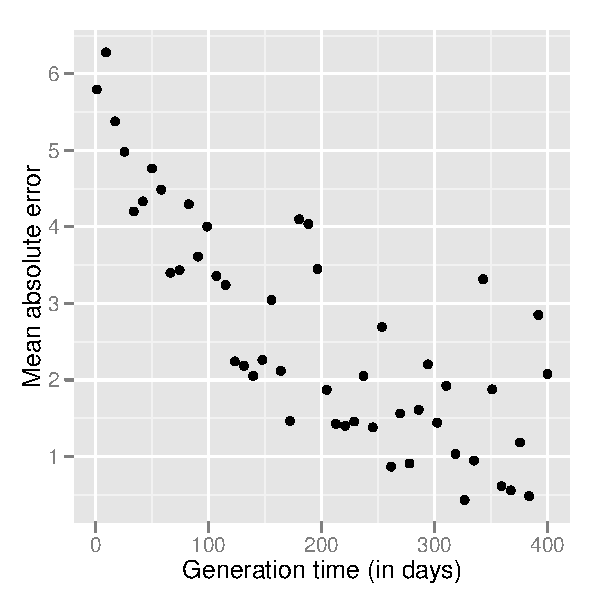
\includegraphics[width=\maxwidth]{figure/hypoth} 
\end{knitrout}

\caption{ \footnotesize{ \textit{Hypothesis  }}\label{fig:hypoth}}
\end{wrapfigure}
\textit{Error analysis} \\
Error can be calculated in three ways: difference in area of occupancy, difference in expanding front, and difference in trailing edge.  The first two are the most common and we will have the largest sample from these.  Because the trailing edge is of the most interest, it can be inferred from total area of occupancy.  Species with less shift in the trailing edge will have a larger total area of occupancy.  All these can be theoretically be compared by converting them to Z-scores and calculating a standard error statistic such as root-mean squared error.  Once we have quantified error, we can construct mixed-effects models with error as the response variable. Using this framework we can add other covariates into our models to control for modeling artifacts, for instance it's known that different SDM contstruction methods have differences in performance \citep{Elith2006, Elith2010}.  Furthermore we will have assembled a database of residual model error.  Our primary goal will be to analyze error in terms of generation time, but this does not exclude considering biotic interactions.  Our group has three experts in networks: mutualistic networks (Chamberlain) and food webs (Poisot, Hart).  Therefore we will also consider mutualistic pairs of species and examine if range shifts are limited by lack of co-expanding mutualists \citep(Hellmann2008, Pelini2010) or enhanced by release from competitive interactions.\\

\textit{Data extraction from figures} \\
Data from SDMs is often presented in the form of distribution maps or scatter plots (Figure 2).  Rather than using existing tools to extract SDM data from figures, we have a more ambitious goal of creating a new tool that we can use within the working group to extract data, and will be a resource for all scientists post-working group.  While tools exist for data extraction from figures, they are all run natively on personal computers. Examples include GraphClick and ImageJ.  We believe a data extraction tool that lives in the web wil be much more powerful and benefit science.  Living in the web, our tool will be cross-platform (Windows, Linux, OSX, etc.), which is extremely important to get wide adoption. In addition, our tool will allow for automatic data retrieval to a database on the backend, presentation of figures called via APIs from various publishers or user uploaded figures, automatic updating of the user interface (UI), authentication of users in order to track user statistics, and other features as needed.  We will build this data extraction tool using a combination of the JavaScript and Python programming languages.  Data will be captured in one of two general ways.
\begin{wrapfigure}{r}{.5\textwidth}
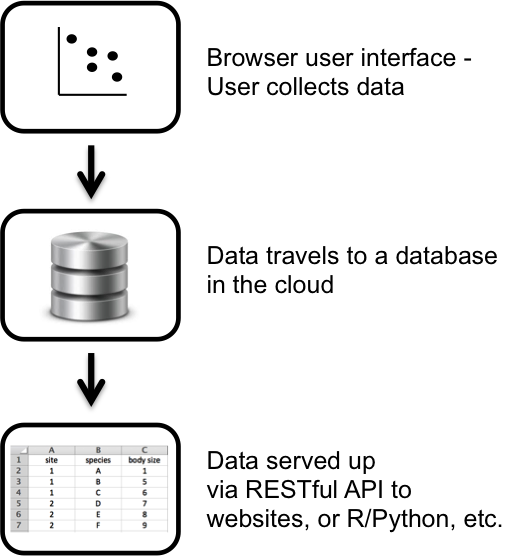
\includegraphics[height=2.2in,width=2.7in]{figextract.png}
\caption{ \footnotesize{ \textit{Figure Extraction  }}\label{fig:figextract}}
\end{wrapfigure}
First, for some figures we will be able to automate data extraction (for an example, see Figure 2).  Second, users will either upload their own figure or will be presented with a figure, at which point they define the axes via clicks on the page, then click on the points of interest on the figure to collect the data.  Instead of the data going to a spreadsheet on a hard drive of a personal computer, the data will all go to a central database stored on servers in the cloud.  Data in the database will be exposed via a RESTful API, which will allow anyone to search and retrieve data.  After or during the NCEAS working group, depending on when the tool is stable, we will beta test the tool with the public to work out bugs.  This tool will eventually allow for crowdsourcing of data extraction from figures at large scales, similar to Galaxy Zoo, Citizen Sky, and FoldIt.  The massive scale at which this tool will operate will transform quantitative meta-analysis studies.  Currently, researchers extract data once from a figure, and someone else may proof their data.  However, with our tool, we can potentially get 10 different users to click on each and every point in a single figure, providing for greater accuracy and a measure of precision.  To make this happen we need a tool that lives in the web and can take advantage of the massive scale at which science can be done. \\

Table 1: \textit{Participant list.  I have organized a group of ecologists, evolutionary bioligists and programmers representing a diversity career stages, institutions and NCEAS experience (* represents new NCEAS visitors.).  In particular all of the programmers are biologists that have experience building computational tools for ecological questions.}\textbf{All listed particpants are confirmed.}
\begin{center}
    \begin{tabularx}{\linewidth}{ | l | l | X |}
    \hline
    \textbf{Participant} & \textbf{Affiliation} & \textbf{Expertise / Notes} \\ \hline
    
    Jessica Hellmann & University of Notre Dame & Climate change, range shifts, adaptation \\ \hline
   
    Lauren Buckley & University of North Carolina Chapel Hill & Climate change, range shifts, SDM development. \\ \hline
    
    Amy Angert & University of British Columbia & Climate change, range shifts, SDM development \\ \hline
     
  Jessica Blois &  University California Merced & Climate change, range shifts SDM development  \\ \hline   
     
  Scott Chamberlain* & Simon Fraser University & Evolution, software development, \textit{NCEAS technical liaison} \\ \hline
  
    Karthik Ram & Univeristy of California Berkeley & Climate change, GIS, software development \\ \hline
 
    Tim Poisot & Université du Québec à Rimouski & Network theory, evolution, software development \\ \hline

  Rich FitzJohn* & The University of New South Wales & Evolution, software development \\ \hline
    
    Jens Stevens* & The University of California Davis & Climate change, range shifts, \textit{Graduate student} \\ \hline 
    
    Mark Hahnel* & Digital Science UK, Figshare & Software development, data management \\ \hline
  
   Edmund Hart* & University of British Columbia & Climate change, software development,        \textit{In charge of data policy requirements} \\ \hline
   
   
   \end{tabularx}
\end{center}



Table 2: \textit{Proposed timeline.  We plan to have three meetings over the course of our working group, each time simultaneously developing our software product and writing manuscripts.}
\begin{center}
    \begin{tabularx}{\linewidth}{ | l | X |}
    \hline
    \textbf{Meeting} & \textbf{Objectives} \\ \hline
    
    Prior to meeting &
    \begin{itemize}
      \item Develop web backend for data extraction from figures, have beta version working.
      \item Create complete list of all relevant SDM papers to extract data from.
      \item Download data for all species in SDM papers and assemble base range sizes and boundaries.
    \end{itemize} \\ \hline
     
     I. December 2012 & 
     \begin{itemize}
      \item Beta test figure extraction software, develop web front end and work with NCEAS to set-up databases to store extracte data.  Begin working on web front-end
      \item Begin extracting data from figures and assembling figure database
      \item Develop models of SDM error.
      \item Create outline for potential manuscripts.
     \end{itemize}
  \\ \hline
       II. Summer 2013 & 
     \begin{itemize}
      \item Complete web front end, and beta user interface for figure extraction.  Work with NCEAS to finalize data storage
      \item Finalize initial manuscripts for submission.
      \item Develop ideas for other uses of the error data extracted from SDMs.
     \end{itemize}
  \\ \hline
       III. Winter 2013 & 
     \begin{itemize}
      \item Publicly release website after any final tweaks.
      \item Revise submitted manuscripts.
      \item Outline and/or make revisions on further manuscripts using our existing data.
     \end{itemize}
  \\ \hline
  \end{tabularx}
\end{center}


\bibliography{NCEASbib}
\end{document}




